\section{Einleitung}

\ac{iot}

\subsection{Motivation}

\begin{displayquote}
  \glqq Wenn Technologien und Gesellschaft sich schneller ändern, als Unternehmen in der Lage sind sich anzupassen, dann kommt es ganz nach den Regeln der Evolution zum Austerben bestimmter Unternehmenstypen.\grqq{}
\end{displayquote}

\begin{flushright}
  \citet[S. 3, zitiert nach Land, K.-H. 2015]{Roth2016}
\end{flushright}

\noindent Die vierte Industrielle Revolution durchläuft zahlreiche Branchen und bringt das Potenzial, sie grundlegend zu verändern. Während einige Branchen und Unternehmenstypen durch die Unterstüzung von \ac{ikt} ihre Effizienz steigern können, sind andere vollständig abhängig von ihnen. Vor allem die Energiewirtschaft ist im Zuge der Energiewende einem grundlgenden Transformationsprozess unterworfen. Durch den Umstieg von Energieproduktionsmethoden wie Kernkraft oder Kohlekraft zu erneuerbaren Energien verlagert sich die Sicht von zentraler Produktion zu dezentraler Produktion. Der Paradigmenwechsel in der Produktion geht in diesem Fall parallel mit dem Pradigmenwechsel in den \ac{ikt} einher. Ohne die technologischen Treiber der Industrie 4.0 wäre die Koordination der dezentralen Anlagen schlichtweg nicht möglich. Im Zeitalter der Digitalisierung nimmt die Geschwindigkeit, in der neue Technologien entwickelt werden rasant zu. Die Technologien als gegeben und ausreichend hinzunehmen, kann sich in Anbetracht des obigen Zitats aus der Sicht aller Branchen als fehlerhaft erweisen. Die Welt wird in ihren kleinsten Komponenten immer mehr vernetzt und nimmt in Entscheidungs- und Steuerungsprozessen ein immer höheres Tempo an. Gleichzeitig steigt mit der Entwicklung der Technologien und der Gesellschaft der Bedarf an Energie. Das Tempo, in dem Entscheidungen getroffen und Steuerungsbefehle gesendet werden, ist besonders in der dezentralen Energieproduktion von existenzieller Bedeutung. Doch die Transformation findet nicht nur von automatisierter zu intelligenter Produktion statt. Der Bedarf an digitalen Dienstleistungen steigt ebenfalls an.  

% Problemstellung
\subsection{Problemstellung} \label{problemstellung}
Monitoring der Sensorwerte einer Windenergieanlage mit SAP-Technologien mit geschlossenem Kreis -> Sensorwerte lösen Aktion wie SMS aus
\newline
Da in der Energiewirtschaft langfristige und teure Investitionsgüter bestehen, können Sie nicht einfach durch neue
digitalisierte Güter ersetzt werden. Umso mehr besteht die Herausforderung, alte Techniken mit neuen Technologien
auf die Digitalisierung vorzubereiten. Wir haben zum Beispiel eine alte Windenergieanlage, die nicht mit den
notwendigen Sensoren ausgestattet sind. Es soll trotzdem ermöglicht werden, Konditionen der Anlage und dessen Umgebung
zu überwachen, um z.B. Wartungsmaßnahmen auszulösen. -> Predictive Maintenance

\begin{itemize}
  \item Technologien zwar bereits im Einsatz aber sind gekapselt -> Insellösungen
  \item Mehrwert durch integrierte Nutzung mit Stammdaten (liegen im SAP System)
  \item SCADA z.B. bereits vorhanden aber Daten nicht intelligent vernetzt
\end{itemize}


\begin{itemize}
  \item[\textbf{FF1}] \textbf{Wie kann SAP Leonardo die digitale Transformation in der Energiewirtschaft mit Internet of Things unterstützen?}
  \begin{itemize}
    \item[FF1.1] Welche Anforderungen an ein System ergeben sich aus Sicht der dezentralen Ernergieerzeugung?
    \item[FF1.2] Welche Möglichkeiten zur intelligenten Vernetzung bietet die zugrundeliegende Systemarchitektur?
    \item[FF1.2] Mit welcher Systemarchitektur können die Anforderungen aus FF1.1 erfüllt werden?
  \end{itemize}
\end{itemize}

\subsection{Lösungsansatz}

Da Energiebranche ausschließlich mit \acf{sapisu} ihre Geschäftsprozesse verwaltet, liegt eine digitale Transformation
mit SAP-Produkten nahe. Dazu wurde ein Raspberry Pi 3 mit entsprechender Sensorik für die Simulation einer Windenergieanlage
ausgestattet. Die gemessenen Werte wurden an den Internet of Things Service der SAP Cloud Platform gesendet und anschlißend
einem digitalen Zwilling übergeben. Um den Zwilling mit entsprechenden Messwerten und Grenzüberschreitungen
sichtbar zu machen, wurde eine SAP UI5-Anwendung entwickelt. Um aus den gemessenen Werten einen Mehrwert zu gewinnen,
wurde ein \acf{aws} \acf{sns} angebunden, der bei Grenzüberschreitung bestimmter Messwerte eine
SMS-Benachrichtigung versendet. All diese Maßnahmen werden prototypisch implementiert

\begin{figure}[ht]
  \centering
  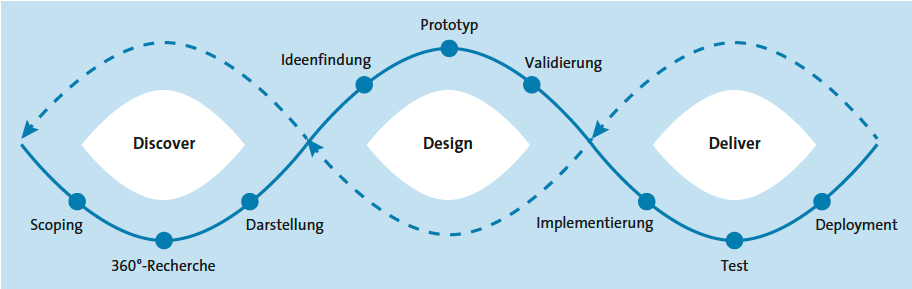
\includegraphics[width=\linewidth]{design_thinking}
  \caption[Phasen des Design-Thinking-Prozesses]{Phasen des Design-Thinking-Prozesses \citep[S. 69]{Elsner2018}}
  \label{}
\end{figure}

\subsection{Aufbau der Arbeit}



\begin{itemize}
  \item Zunächst Industrie 4.0 und treibende Faktoren allgemein
  \item Was ist der Mehrwert von Kommunikationssystemen und welche Protokolle sind Grundlage für die Vernetzung?
  \item Welche Referenzarchitektur vereinheitlicht industrielle Standards und Anforderungen an die Systeme?
  \item Was ist Cloud Computing und welche Rolle spielen dessen Technologien für Industrie 4.0?
  \item Welche Toolsets sind für die Lösung vorhanden?
  \item Use Case: Für welchen Anwendungsfall in der Energiebranche wird ein Prototyp entwickelt?
  \item Was sind die Anforderungen an den Prototypen? Näherer Bezug auf Energiebranche.
  \item Welche Komponenten besitzt das entworfene System bzw. sind notwendig?
  \item Wie sieht die Implementierung im Detail aus?
  \item Evaluierung des Vorgehens
  \item Fazit
\end{itemize}



\newpage
